\documentclass{article}

% packages -> http://www.howtotex.com/packages/9-essential-latex-packages-everyone-should-use/
\usepackage[utf8]{inputenc}
\usepackage{hyperref}
\usepackage{amsmath,amssymb,amsthm,amsfonts,mathtools,mathrsfs}
\usepackage{tocbibind}
\usepackage{bbm}
\usepackage{enumitem}
\usepackage{fancyhdr}			% per i numeri di pagina
\usepackage[a4paper,margin=0.8in]{geometry}	% to adjust the margins of pages
\usepackage{graphicx}			% for inserting figures
\usepackage{microtype}			% document reads better
% \usepackage[backend=bibtex,style=numeric]{biblatex}
\usepackage[toc]{appendix}
\usepackage{todonotes}
\usepackage{geometry}
\usepackage{subfigure}
\usepackage{algorithm}
\usepackage[noend]{algpseudocode}
\usepackage{listings}
\usepackage{color}
\usepackage{caption}

\newcommand{\inputfrom}[1]{\input{./tex/#1/#1}}

\setcounter{MaxMatrixCols}{30}
\providecommand{\U}[1]{\protect\rule{.1in}{.1in}}
\newtheorem{theorem}{Theorem}
\newtheorem{acknowledgement}[theorem]{Acknowledgement}
\newtheorem{axiom}[theorem]{Axiom}
\newtheorem{case}[theorem]{Case}
\newtheorem{claim}[theorem]{Claim}
\newtheorem{conclusion}[theorem]{Conclusion}
\newtheorem{condition}[theorem]{Condition}
\newtheorem{conjecture}[theorem]{Conjecture}
\newtheorem{corollary}[theorem]{Corollary}
\newtheorem{criterion}[theorem]{Criterion}
\newtheorem{definition}[theorem]{Definition}
\newtheorem{example}[theorem]{Example}
\newtheorem{exercise}[theorem]{Exercise}
\newtheorem{lemma}[theorem]{Lemma}
\newtheorem{notation}[theorem]{Notation}
\newtheorem{problem}[theorem]{Problem}
\newtheorem{proposition}[theorem]{Proposition}
\newtheorem{remark}[theorem]{Remark}
\newtheorem{solution}[theorem]{Solution}
\newtheorem{summary}[theorem]{Summary}

\graphicspath{ {img/} }

\DeclarePairedDelimiter\ceil{\lceil}{\rceil}
\DeclarePairedDelimiter\floor{\lfloor}{\rfloor}

\renewcommand*\thelstnumber{\arabic{lstnumber}:}

\DeclareCaptionFormat{mylst}{\hrule#1#2#3}
\captionsetup[lstlisting]{format=mylst,labelfont=bf,singlelinecheck=off,labelsep=space}

\definecolor{mygreen}{rgb}{0,0.6,0}
\definecolor{mygray}{rgb}{0.5,0.5,0.5}
\definecolor{mymauve}{rgb}{0.58,0,0.82}

\lstset{ %
  backgroundcolor=\color{white},   % choose the background color; you must add \usepackage{color} or \usepackage{xcolor}; should come as last argument
  basicstyle=\footnotesize,        % the size of the fonts that are used for the code
  breakatwhitespace=false,         % sets if automatic breaks should only happen at whitespace
  breaklines=true,                 % sets automatic line breaking
  captionpos=b,                    % sets the caption-position to bottom
  commentstyle=\color{mygreen},    % comment style
  deletekeywords={...},            % if you want to delete keywords from the given language
  escapeinside={\%*}{*)},          % if you want to add LaTeX within your code
  extendedchars=true,              % lets you use non-ASCII characters; for 8-bits encodings only, does not work with UTF-8
  frame=single,	                   % adds a frame around the code
  keepspaces=true,                 % keeps spaces in text, useful for keeping indentation of code (possibly needs columns=flexible)
  keywordstyle=\color{blue},       % keyword style
  language=C,              		   % the language of the code
  morekeywords={*,...},            % if you want to add more keywords to the set
  numbers=left,                    % where to put the line-numbers; possible values are (none, left, right)
  numbersep=5pt,                   % how far the line-numbers are from the code
  numberstyle=\tiny\color{mygray}, % the style that is used for the line-numbers
  rulecolor=\color{black},         % if not set, the frame-color may be changed on line-breaks within not-black text (e.g. comments (green here))
  showspaces=false,                % show spaces everywhere adding particular underscores; it overrides 'showstringspaces'
  showstringspaces=false,          % underline spaces within strings only
  showtabs=false,                  % show tabs within strings adding particular underscores
  stepnumber=2,                    % the step between two line-numbers. If it's 1, each line will be numbered
  stringstyle=\color{mymauve},     % string literal style
  tabsize=2,	                   % sets default tabsize to 2 spaces
  title=\lstname                   % show the filename of files included with \lstinputlisting; also try caption instead of title
}

\hypersetup{
    backref,
    bookmarks=true,         % show bookmarks bar?
    unicode=false,          % non-Latin characters in Acrobat’s bookmarks
    pdftoolbar=true,        % show Acrobat’s toolbar?
    pdfmenubar=true,        % show Acrobat’s menu?
    pdffitwindow=false,     % window fit to page when opened
    pdfstartview={FitH},    % fits the width of the page to the window
    pdftitle={Network of interacting neurons with random synaptic weights},    % title
    pdfauthor={Grazieschi Paolo \& Leocata Marta \& Mascart Cyrille},     % author
    pdfsubject={Study of the mean-field equation of a network of interacting leacky integrate and fire neurons},   % subject of the document
    pdfcreator={Grazieschi Paolo \& Leocata Marta \& Mascart Cyrille},   % creator of the document
    pdfproducer={Grazieschi Paolo \& Leocata Marta \& Mascart Cyrille}, % producer of the document
    pdfkeywords={neurons, mean-field, fokker-planck, stochastic process}, % list of keywords
    pdfnewwindow=true,      % links in new PDF window
    colorlinks=true,       % false: boxed links; true: colored links
    linkcolor=red,          % color of internal links (change box color with linkbordercolor)
    linkbordercolor=white,
    citecolor=green,        % color of links to bibliography
    filecolor=magenta,      % color of file links
    urlcolor=cyan,           % color of external links
    urlbordercolor=white
}

\captionsetup{compatibility=false}
\DeclareCaptionSubType*{algorithm}
\renewcommand\thesubalgorithm{\thetable\alph{subalgorithm}}
\DeclareCaptionLabelFormat{alglabel}{Alg.~#2}

\algnewcommand\algorithmicto{\textbf{to}}
\algrenewtext{For}[3]{%
  \algorithmicfor\ #1 $\gets$ #2 \algorithmicto\ #3 \algorithmicdo
}
\algnewcommand\COMMENT[2][.1\linewidth]{%
  \leavevmode\hfill\makebox[#1][l]{$\triangleright$~#2}
}
\algnewcommand\RETURN{\State \textbf{return} }

\tikzstyle{vecArrow} = [thick, decoration={markings,mark=at position
   1 with {\arrow[semithick]{open triangle 60}}},
   double distance=1.4pt, shorten >= 5.5pt,
   preaction = {decorate},
   postaction = {draw,line width=1.4pt, white,shorten >= 4.5pt}]
\tikzstyle{innerWhite} = [semithick, white,line width=1.4pt, shorten >= 4.5pt]

\renewcommand{\d}[1]{\ensuremath{\operatorname{d}\!{#1}}}

\everymath{\displaystyle}
%\usepackage{indentfirst}
%\setlength{\parindent}{1cm}

\begin{document}
		\indent In this section we are going to develop an algorithm for the simulation of neurons the potentials of which are modeled with a mean-field equation. In this case the equation is the result of a limit approximation of the behaviour of an infinite network of integrate and fire neurons. In order to obtain relevant simulation results one should consider the means to simulate a network as big as possible. Not only to get closer to the infinite network hypothesis but also because the number of neurons in biological brains is typically huge: a drosophilia for instance has a number of neurons of order $2.55\times10^5$, while for human beings this number verges on the 90 billions - and it gets even higher for bigger animals like elephants or whales.\\\indent
	\section{Simulated model}\label{sec:model}
		\indent First, we need to discuss about some choices that were made about the model. As a reminder, the potential of the neurons follows the mean-field equation:\\\indent
		\begin{equation}
			\forall i\in\{1,\cdots,N\}, V_i(t)=V_i(0)+\int_0^t b(V_i(s))ds+\sigma W_t+\sum_{j=1}^NJ_{j\to i}M_{j,t}-M_{i,t}(V_{i,T}-V_{i,R})
		\end{equation}
		where,\begin{align*}
			V_i			& \text{ is the membrane potential of the neuron i}\\
			b			& :\mathbb{R}_{+}\to\mathbb{R}_+\text{ is a drift, and is a lipschitz function of the potential}\\
			W_t			& \text{ is a Brownian motion}\\
			M_{i,t}		& =\sum_k\delta(t-T_{i,k})\text{, where }\delta\text{ is the Dirac Delta at zero and}\\
						& \indent T_{i,k}\text{ is the times of the }k^{th}\text{-spike coming out of the neuron i}\\
			J_{j\to i}	& \text{ is the synaptic weight of the connection from j to i}\\
			V_{i,T}		& \text{ is the membrane's potential threshold of the neuron i}\\
			V_{i,R}		& \text{ is the reset value of the membrane potential after spiking of the neuron i}
		\end{align*}
		The $(V_i)_{i\in\{1,\cdots,N\}}$ are discontinuous functions of time, and the discontinuities represent neurons spiking in the system. By simulating this system of neurons we are interested in finding what parameter set creates a given pattern, and more specifically a blow-up of the system, when at a given time the spiking rate tends to infinity.\\\indent
		A spike is an abstract and instantaneous event marking a reset of the potential for the spiking neuron and change in potential for postsynaptic neurons. A neuron i can emit a spike only if its potential is higher than the threshold $V_{i,T}$. The choice has been made to consider the spikes as point processes, with the probability of having a spike depending on the potential of the neuron. Here we must introduce the function $f:\mathbb{R}\to\mathbb{R}_{+,*}$ that will be used to compute the spiking probability. f is defined so that:\\\indent
		\begin{equation*}
			f:	\begin{aligned}
					\mathbb{R}&\to&&\mathbb{R}_{+}\\
					x&\mapsto&&f(x)=C\times\text{Pos}(x-V_T)^p
				\end{aligned}
		\end{equation*}
		where C and p are constants (actually $C>>1$) and Pos is defined so that:
		\begin{equation*}
			\text{Pos}:	\begin{aligned}
							\mathbb{R}&\to\mathbb{R}_+\\
							x&\mapsto Pos(x)=	\begin{cases}
													x\quad\text{if }x>0\\
													0\quad\text{otherwise}
												\end{cases}
						\end{aligned}
		\end{equation*}
		This function is used in the rejection-sampling algorithm explained in section~\ref{sec:rejectionsampling}. It is equal to zero for values of the potential below the threshold, as biological neurons do not spike when their potential is below such a threshold (well, actually it depends on the type of neurons we are dealing with, but this is mostly true for cortex neurons). When the potential exceeds the threshold, the probaility of spiking should quickly increase so that the neuron will quickly spike.\\\indent
		Also an important function is the approximation function \~f defined as:
		\begin{equation*}
			\text{\~f}:	\begin{aligned}
							\mathbb{R}^3&\to\mathbb{R}_+\\
							(x,[A,B])\mapsto\text{\~f}(x,[A,B])=\max_{x\in[A,B]}(f(x))
						\end{aligned}
		\end{equation*}
		There are several reasons for the choice of a probability of spiking and not a deterministic condition. First, even if there is still a kind of threshold, this model opens the possibility for simulating neurons with a softer threshold (or even no threshold at all if $\forall i\in\{1,\cdots,N\}, V_{i,T}=0$). But the most important reason is actually to avoid having no solution at blow-up time because of an infinite amount of spikes at that time. This is interesting for studying the long-term behaviour of such a system.\\\indent
		In short, we are interested in discrete abstract events marquing discontinuities in the neurons' membranes potential. These events appear at random, following a distribution that is function of this membrane potential. These are important considerations, because they make explicit the kind of algorithm we need. From now on, these discontinuities will be named spikes or events indifferently.\\\indent
		The reset value $V_{i,R}$ is the value of the potential of the neuron i just after a spike. It is obviously smaller than the threshold value, but the difference between the two is important because it influences how much time a neuron must wait after a spike for being able to spike again. In biological neurons there is what is called a refractory period, which is not modelled here, during which a neuron cannot spike after having emmited a spike. The potential of a neuron in such state is very low, actually lower than the value of the potential at rest. It is fixed at 0, to be compared to 1 for the threshold.\\\indent
		The synaptic weights $(J_{j\to i})_{(i,j)\in\{1,\cdots,N\}^2}$ are the amount by which the potential of a neuron i children of neuron j changes when j spikes. The $M_{i,t}$ are the history of neurons, that is to say how many times the neuron i has spiked.\\\indent
		Finally the $b:\mathbb{R}_{+}\to\mathbb{R}_+$ function makes the neurons naturally proned to spike, as it makes the neurons potentials tend to a given value, higher than the threshold. b is defined as:
		\begin{equation*}
			b:	\begin{aligned}
					\mathbb{R}_+\to\mathbb{R}
					x\mapsto b(x)=-\lambda(x-a), (\lambda,a)\in\mathbb{R}_+^2
				\end{aligned}
		\end{equation*}
	\section{Rejection sampling algorithm}\label{sec:rejectionsampling}
		Here we present the actual algorithm developed for the simulation of the model presented above. Discussions about its complexity and its actual implementations can be found in sections~\ref{sec:complexity}~and~\ref{sec:implementation}.\\\indent
	\subsection{Clock-driven vs. event-driven algorithm}
		\indent The classical way of solving a differential equation is to define a time step $\Delta t$ and then use a numerical method (Runge-Kutta or linear multistep) for recursively solving with $y(t+\Delta t)=f(Y(t))$. These methods usually give good approximations of the exact solution, while being quite simple to implement. They are however time expensive, because of the value $\Delta t$ that must be small enough for not missing any quick variations of the solution.\\\indent
		Event-driven simulations on the contrary optimises the computations to focus on events, computing the state of the system only when they occur. What are events is an arbitrary choice, but most of the times they represent a change in the system dynamic (variation in the derivative, discontinuities, etc).\\\indent
		As we are going to explore the spiking behaviour of a network of neurons, the second option comes naturally. This method is also very natural when considering a stochastic system, with events like spikes appearing at random with a non common distribution, so that a rejection sampling method is necessary for getting the events.\\\indent
	\subsection{The algorithm}
		\begin{algorithm}
			\begin{algorithmic}[1]
				\State N: number of neurons
				\State \~T: time elapsed since last event in the system
				\State $T_{last}$: absolute time of the last event in the system
				\State $T_{next}^i$: absolute time of the nth event of neuron i
				\State $\mathscr{P}$: poisson distribution
				\State $\mathscr{U}$: uniform distribution
				\State \~f: approximation function of function f (\~f$(x)\ge f(x)$)
				\Repeat
					\Repeat\COMMENT{Steps 0-1}
						\State determine an interval $[A,B[$ on which sampling
						\State compute the array of $(\text{\~f}_i(V_i(A)))_{i\in\{1,\cdots,N\}}$ and $\sum_i\text{\~f}_i(V_i(A))$ on interval $[A,B[$
						\State \~T$\sim\mathscr{P}(\lambda=\sum_i\text{\~f}_i)$
						\State $T_{next}\gets T_{last}+$\~T
					\Until{in good interval AND at least one $\text{\~f}_i\neq0$}
					\State $i\gets\textbf{argmin}_{i\in\{1,\cdots,N\}}\left(\sum_j \text{\~f}_j(V_j(A)) * u\sim\mathscr{U}([0,1])<\text{\~f}_i(V_i(A))\right)$\COMMENT{Step 2}
					\State $T_{i,n}\gets T_{next}$\COMMENT{Step 3}
					\State $V_i(T_{i,n})\gets a+e^{-\lambda\text{\~T}}(V_i(T_{i,n-1})-a)+\sigma\mathscr{N}(0,\frac{1-e^{-2\lambda\text{\~T}}}{2\lambda})$
					\State $\mathbb{P}(\text{accepting spike of neuron i})=\frac{f_i(V_i(T_{i,n}))}{\text{\~f}_i(V_i(A))}$\COMMENT{Step 4}
					\If{spike is accepted}
						\State update potentials of all postsynaptic neurons
					\EndIf
				\Until{an end condition is met}
			\end{algorithmic}
			\caption{Simulator}\label{alg:rejacc}
		\end{algorithm}
		\indent The algorithm is presented in figure~\ref{fig:rejacc}. It explicits the several steps for simulating the network of neurons.\\\indent
		The main idea here is the rejection sampling method for finding the spikes. This method is applied as many times as necessary for reaching a certain condition, typically a number of spikes found. The actual sampling is made at step 4, but several steps are necessary before being able to sample events.\\\indent
		The first step (0) is looking for a time interval, where the next event shall be looked for. This step is actually important for the speed of the algorithm, as bounding the time also makes possible to derive a better approximation for the approximation functions \~f$_i$. The separation between two sequential events follow a Poisson distribution of parameter the sum of the approximation functions (step 1):
		\begin{equation}
			T_{k+1}=T_k+\text{\~T}\text{, with \~T}\sim\mathscr{P}(\sum_i\text{\~f}^i)
		\end{equation}
		This step gives the time when the event is occuring, and now the neuron responsible for the event must be found. The sum of the approximation functions is used again, as the probability of having a spike depends on them. The bigger the value of \~f$_i$, the higher the probability that the neuron i will be the next spiking. A random number, uniformly distributed, choses the winner.\\\indent
		Knowing which neuron is having an event and at what time it is then possible to update its potential $V_i(T_{next})$ (step 3). It is important to remark that if the event was until now categorised as $T_{next}$, it is now differentiated as an event of neuron i (2 in the figure). An event in the system is indeed linked to the neuron having this event, but the same neuron is usually not responsible for two consecutive events in the system. That is why $T_{last}$ is not equal to $T_{2,n-1}$ in the figure: $T_{last}$ is the last event in the system (caused for instance by neuron 1), while $T_{2,n-1}$ is the last event of the neuron 2.\\\indent
		The value at time $T_{i,n}$ of $V_i$ was necessary for computing the value of the probability function f$_i(V_i(T_{i,n}))$ and thus classifying the event between false and true spike (step 4). The value of a random variable uniformly distributed between 0 and \~f gives the classification: if its lesser than $f(V_i(T_{i,n}))$ the spike is a true one, greater its a false one. If the spike is a true one the potential of the spiking neuron is reset to $V_{i,R}$ while the potentials of all the postsynaptic (children) neurons are updated to the time of event $T_{next}$. The value of the synatic weight $J^{i\rightarrow j}$ is then added to their potential (possibly making them reach their threshold). If the spike was a false one, nothing happens.\\\indent
		The algorithms then loops back to step 0 until a given condition (number of spikes reached, time elapsed, etc.) is met.\\\indent
	\section{Graph management}\label{sec:graph}
		\begin{algorithm}
			\begin{algorithmic}[1]
				\State RNG: Random Number Generator
				\State p: Probability of connection between two neurons
				\State $\mathscr{M}_{i,j}$: matrix of interaction: equals 1 for a connection, 0 otherwise
				\State \Call{RNG.B}{p}: returns 0 or 1, bernouilli distributed with probability p.
				\Function{Interaction matrix}{RNG, p}
					\For{i}{1}{n}
						\For{j}{1}{n}
							\State $\mathscr{M}_{i,j}\gets$\Call{RNG.B}{p}
						\EndFor
					\EndFor
				\EndFunction
			\end{algorithmic}
			\caption{Generation of a matrix of children}\label{alg:mat}
		\end{algorithm}
		Algorithm~\ref{alg:mat} is the classical algorithm used for creating an Erd\"os-Renyi directed graph. It is composed of two loops, looking at all pairs (i,j) of neurons. The probability of having a connection between these two neurons (and from i to j) is Bernouilli of a constant parameter p. At each call of the RNG, a random value Bernouilli distributed is thus created and the status of the RNG changes from $S_k$ to $S_{k+1}$. The result of whether there is a connection or not between two neurons is stored in a matrix called interaction matrix, of values equal to 1 if there is a connection and 0 otherwise. This matrix can be huge in the case where there are a great number of connections, as its size is of order the number of neurons squared. Even if only the relevant parts of the matrix are actually stored (meaning the ones of the matrix), the size is still of order $pN^2$. That means for instance the graph of a network of $N=10^5$ neurons needs at maximum $10^{10}$ storage units (bits, bytes, etc.), which is beyond the amount of memory typically available in most personnal computers nowadays.\\\indent
		\begin{algorithm}
			\begin{algorithmic}[1]
				\State RNG: random Number Generator
				\State p: probability of connection between two neurons
				\State N: number of neurons in the system
				\State S: vector of pairs (Status of the RNG, Number of children of neuron i)
				\State \Call{RNG.Bin}{N,p}: returns a random value following the binomial distribution of parameter N and p
				\State \Call{RNG}{$S_i$}: returns the index of a child for i among all other unchosen neurons
				\State \Call{RNG.Status}{}: returns the current internal state of the RNG
				\State $I_i$: number of children of neuron i
				\Function{Make vector}{RNG, p}
					\For{i}{1}{N}
						\State $I_i\gets$\Call{RNG.Bin}{N,p}
						\State $S[i]\gets$(\Call{RNG.Status}{},$I_i$)
						\For{j}{1}{$I_i$}
							\State\Call{RNG}{S$_{j+\sum_{k=1}^{i-1}I_k}$}
						\EndFor
					\EndFor
				\EndFunction
			\end{algorithmic}
			\caption{Generation of a vector of rng states}\label{alg:vect}
		\end{algorithm}
		So another idea would be to "compress" the data so that it takes less space, and the convenient thing here is that when looking up closely to the classical generation method, the data of the matrix is already compressed in the state of the RNG at the beginning of the algorithm. The compression rate is great, but usability is really bad, because in order to access to any connection value one would have to reconstruct a great part of the matrix before. A middle way solution is the one presented by algorithm~\ref{alg:vect}, where the idea of using the RNG state as a compression of the interaction matrix can be extended further to compress not the whole matrix but only its rows, or the children of the neurons to say it otherwise.\\\indent
		First, the graph must be generated the same way it is done in the classical method. But instead of storing, for each child j of the neuron i, the value of the connection in a matrix, we just remember that associated to i is the state $S_i$ of the RNG. Then for each child j the value of the connection is generated in a classical way, except for the storing in a matrix part.\\\indent
		\begin{algorithm}
			\begin{algorithmic}
				\Function{Comparison}{}
					\State \Call{Interaction Matrix}{$RNG_1$,p}
					\State \Call{Make Vector}{$RNG_2$,p}
					\State \hspace{1.5cm}$\vdots$ Simulation
					\State \textbf{Neuron i is spiking}
					\State $\triangleright$ Using matrix graph
						\For{j}{1}{N}
							\If{$\mathscr{M}_{i,j}=1$}
								\State Update potential of neuron j
							\EndIf
						\EndFor
					\State $\triangleright$ Using reconstruction
						\State S[i]=(S$_{\sum_{k=1}^{i-1}I_k},I_i$)
						\State \Call{RNG.SetState}{S[i][1]}
						\For{j}{1}{$I_i$}
							\State Child$_j\gets$\Call{RNG}{S$_{j-1+\sum_{k=1}^{i-1}I_k}$}
							\State Update potential of neuron Child$_j$
						\EndFor
				\EndFunction
			\end{algorithmic}
			\caption{Comparison of usage between clasical method and reconstruction}\label{alg:comparison}
		\end{algorithm}
		The reason why this method is really effective in our case is that whenever a neuron spikes, we have to update the potential of all of its children. The value of the connectivity between two specific neurons is actually never wanted, and so the matrix-based method and the reconstruction-based method will both be used in a similar fashion, that is, for a given neuron i, make something with all its children. Hence the loop on all the children in the comparison algorithm~\ref{alg:comparison}.\\\indent
		A question raises then that is the question of the complexity of such a reconstruction-based method compared to the complexity of the classical one. This is a broader matter actually that must be extended to all that have been previously presented here, and so it deserves its own section.\\\indent
	\section{Complexity: memory and instructions}\label{sec:complexity}
		\begin{definition}[Algorithmic complexity]
			Analysis of algorithms is the domain interested in determining the amount of resources, may they be time, storage or other resources, necessary in order to execute a given algorithm. Usually the idea is to find a function relating the input of an algorithm to to the number of steps it takes (its time complexity) or the number of storage locations it uses (its space complexity). Most of the time the complexity is examined in the asymptotic sense, in other word, how much of a resource do one need in order to run the algorithm when the input's size grows to infinity? The Big O notation is then used.
		\end{definition}
		The use of the Big O notation is not insignificant, as this means that two algorithms with the same order of complexity (or two implementations of the same algorithm) may execute with very different amount of resource because there may exist a significant factor between the two (that will become unsignificant asymptotically, but not for small inputs). Knowing this limitation, this kind of analysis focus more on differences of the orders of complexity between two algorithms/implementations.\\\indent
		\begin{table}
				\begin{tabular}{|c|c|c|c|}
						\hline
													&	Time complexity at creation		&	Time complexity during usage	&	Space complexity	\\\hline
						Reconstruction method		&	$\mathscr{O}(N\times\max(I_i))$	&	$\mathscr{O}(\max(I_i))$		&	$\mathscr{O}(N)$	\\\hline
						Interaction matrix			&	$\mathscr{O}(N^2)$				&	$\mathscr{O}(1)$				&	$\mathscr{O}(N^2)$	\\\hline
						%Interaction list			&	$\mathscr{O}(N^2)$				&	$\mathscr{O}(N)$				&	$\mathscr{O}(N^2)$	\\\hline
				\end{tabular}
			\caption{Table of time and memory complexity. $I_i$ refers as before to the influencees of the neuron i}\label{tab:complexity}
		\end{table}
		The first complexity is given as an example of how the complexity is computed. In the classical algorithm for generating an interaction matrix, for all potential parent,one must look at all the other neurons in order to determine whether they are a child of the first one. Hence the double loop on all neurons, for looking at all the elements of the interaction matrix. In the case of the reconstruction method presented above, the number of children of a given parents is determined before hand, and in the second loop their index.\\\indent
		This is the method that is actually used for another type of graph storage structures, called interation list (they have a space complexity similar to interaction matrices, so we are not discussing them here), at it allows to gain some time at the creation and space in memory.\\\indent
		It is interesting to note that as the only input of the algorithm (at least the only asymptotically relevent input) is the number of neurons, everything that is constant in regards to this number does not appear in the complexity. For intance, the random number generation takes time, but as it is constant in regards to the number of neurons it does not appear in the final computation of the complexity.\\\indent
		Finally for the first column, one should take care that even if the time complexity at creation of the reconstruction method is lower than the complexity of the interation matrix in practice, this is not the case theoretically, as one should always look for the worst case scenario, that is the complete graph in this case. In this scenario, any neuron has all neurons (including self) as children, and so $\max(I_i)=N$.\\\indent
		The interesting parts in this table are the last two columns. The space complexity is obviously where the method shines the most, as it helps gain at least an order of magnitude, making it very relevant for storing very big graphs. On the other hand, the time complexity using the vector of RNG states is worse than the time complexity of using the interaction matrix, but as shown in the example algorithm~\ref{alg:comparison}, as we are only interested in manipulating the children (and all of them at the same time), the complexity of using the interaction matrix in our case would have been $\mathscr{O}(N)$ anyway, so the method is very interesting at usage.\\\indent
		The figure~\ref{fig:complexity} exposes the differencces in complexity between an event-driven algorithm (in blue) and a clock-driven algorithm (in red). 
		The complexity of clock-driven algorithms is of order $N^2$. Event-driven algorithms have much less complexity, of order N. But as our algorithm is based on a thinning method, the complexity is higher, but still linear of N.\\
	\section{Implementation}\label{sec:implementation}
		The algorithm was first prototyped using Java and the final implementation was produced in C. Using higher level languages often poses issues with his kind of problematics as they tend to trade scarcity in resource cnsumption for easiness of use. Also using compiled languages opens the door of compiler optimisations with greatly improved speed and memory.\\\indent
		About memory consumption, the representation of numbers, especially real numbers, is a big issue when dealing with this kind of algorithms. There are indeed both very big and very small numbers used at the same time during the simulation. Summing the values of all the approximation functions ($10^5$ values) could lead to overflow, that is a lack of bits for correctly representing the number. Different languages uses different ways of overcoming this kind of limitations, depending on which standard is actually implemented. For Java it is the IEEE 754 binary floating point representation, which makes possible to represent floating point numbers with at least 15 digits of precision (not accuracy). For C it really depends on the floating point type chosen.
	\subsection{A word about the rng}
		The Random Number Generator is a very important component of the algorithms described above and the choice has been made of using the well known Mersenne-Twister, which can provide high quality integer or floating point ranodm numbers. The version we used is the one developped and maintained by the creator of the Mersenne-Twister himself, Makoto Matsumoto, and can be found at \url{http://www.math.sci.hiroshima-u.ac.jp/~m-mat/MT/SFMT/index.html}.\\\indent
		A related subject is the distribution followed by the random numbers. The algorithm presented earlier needs several random numbers from various distributions, none of them being too exotic (uniform numbers with arbitrary upperbound and normal numbers centered on zero with arbitrary variance), but as the library used only provide uniform random series of 32 or 64 bits and random floating point numbers in [1,2) or {[0,1], [0,1), (0,1], (0,1)}, we must implement a way to generate the numbers drawn from our arbitrary distributions. In both cases a sampling method (again) is used, and we are going to describe them.\\\indent
		First the uniform case. We have a random integer generator, and we assume it gives perfectly random numbers in $ {0, 1, ..., M} $, while we want uniform numbers in $ {0, 1, ..., U} $. A common method to achieve this is to use a modulo: $ \mathbb{U}([0, M]) mod[U+1] $. The issue here is that unless M is a multiple of $ U+1 $, the uniformity of the numbers is lost using this method. The case in which the method works can be used as a trick for guarrantying uniformity though. Indeed, if M is not a multiple of $ U+1 $, there must exist one that is lower than M but close anyway. Knowing that, we can simply take any number that is lower than $ U+1 $ and in the rare cases a number greater than $ U+1 $ is drawn, we just have to reject it and draw another one.\\\indent
	\subsection{Improving speed}
		With the increase of the number of computers having several cores, it becomes more and more interesting to design algorithms with the possibility to use parallelisation for speeding them. Yet, this is not really possible for some of them, and here the main loop of the rejection sampling method exposed in section~\ref{sec:rejectionsampling} is a good example. Finding the next event time relies on the sum of the approximation functions, which indirectly depend on the potential of each neuron which is computed at the previous event. But if this sequential part cannot be parallelised, some other time consuming parts can!\\\indent
		There is indeed a lot of computations involving large arrays of numbers, be it the computation of the approximation functions for all neurons or the update of the potential of all children neurons. Thanksfully a lot of tools exist that answer this problematic, and one very adapted to our problem is openmp, which is the solution used for the implementation. This solution is also compatible with the parallelisation of the reconstruction method: instead of storing one state of the RNG per parent neuron, one could sample the state several times during the graph generation. For instance storing the state every 100 children neurons instead of one time. The different states can be used to instanciate several parallel RNGs that will recreate the children in parallel.\\\indent 
		There are also solutions for speeding the random number generation by directly generating streams of random numbers instead of on number at a time, again relying on the possibility to parallelise such generation.\\
		
		Finally, there is one parameter that have not been discussed while having a certain importance on the speed of the algorithm, it is the [A,B[ interval, step 0 of the algorithm in figure~\ref{fig:rejacc}. The smaller the length of this interval the closer the approximation function \~f if of the probability function f. But when the length of the interval is too small, then the time of events, Poisson generated, are greater than the upper-bound of the interval, leading to frequent change in the interval (and the algorithm comes closer to the time complexity of clock-driven algorithms). Finding an optimal here is a difficult issue because the size of the interval depends on the expected value of the Poisson distribution which is the sum of the approximation function computed on the interval [A,B[$\cdots$
		\begin{landscape}
			\begin{figure}
				\begin{center}
					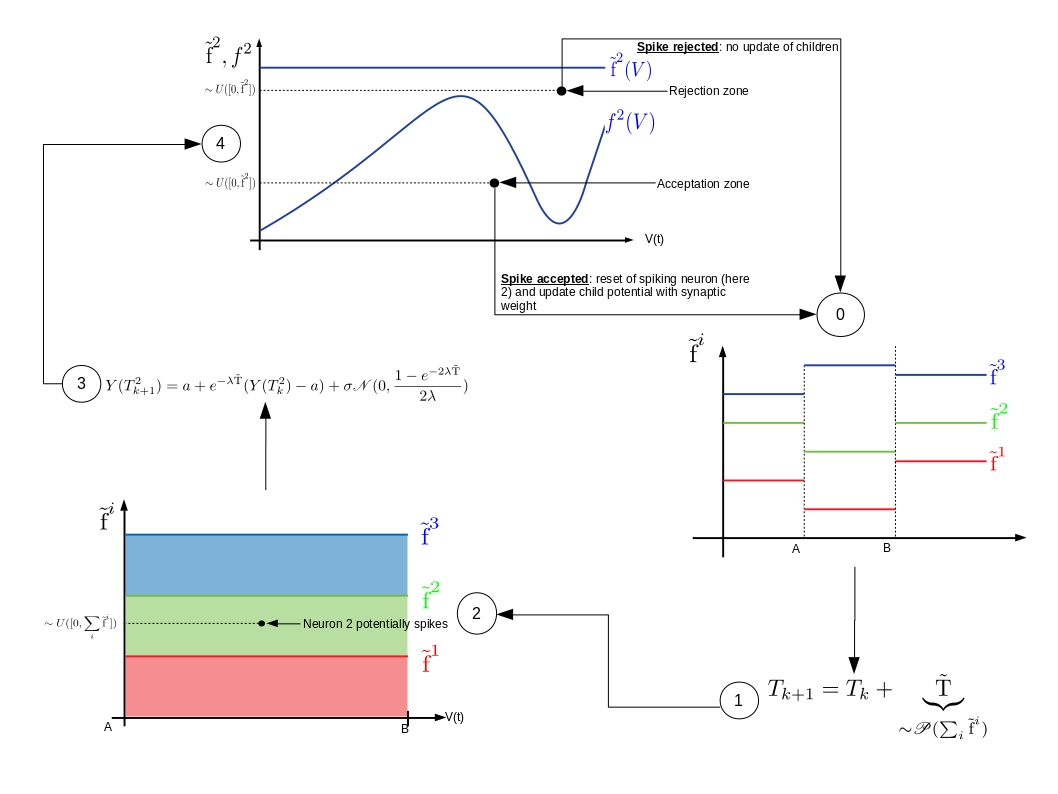
\includegraphics[width=\linewidth]{rejectaccept}
				\end{center}
				\caption{Illustration of algorithm~\ref{alg:rejacc}}\label{fig:rejacc}
			\end{figure}
		\end{landscape}
		\begin{landscape}
			\begin{figure}
				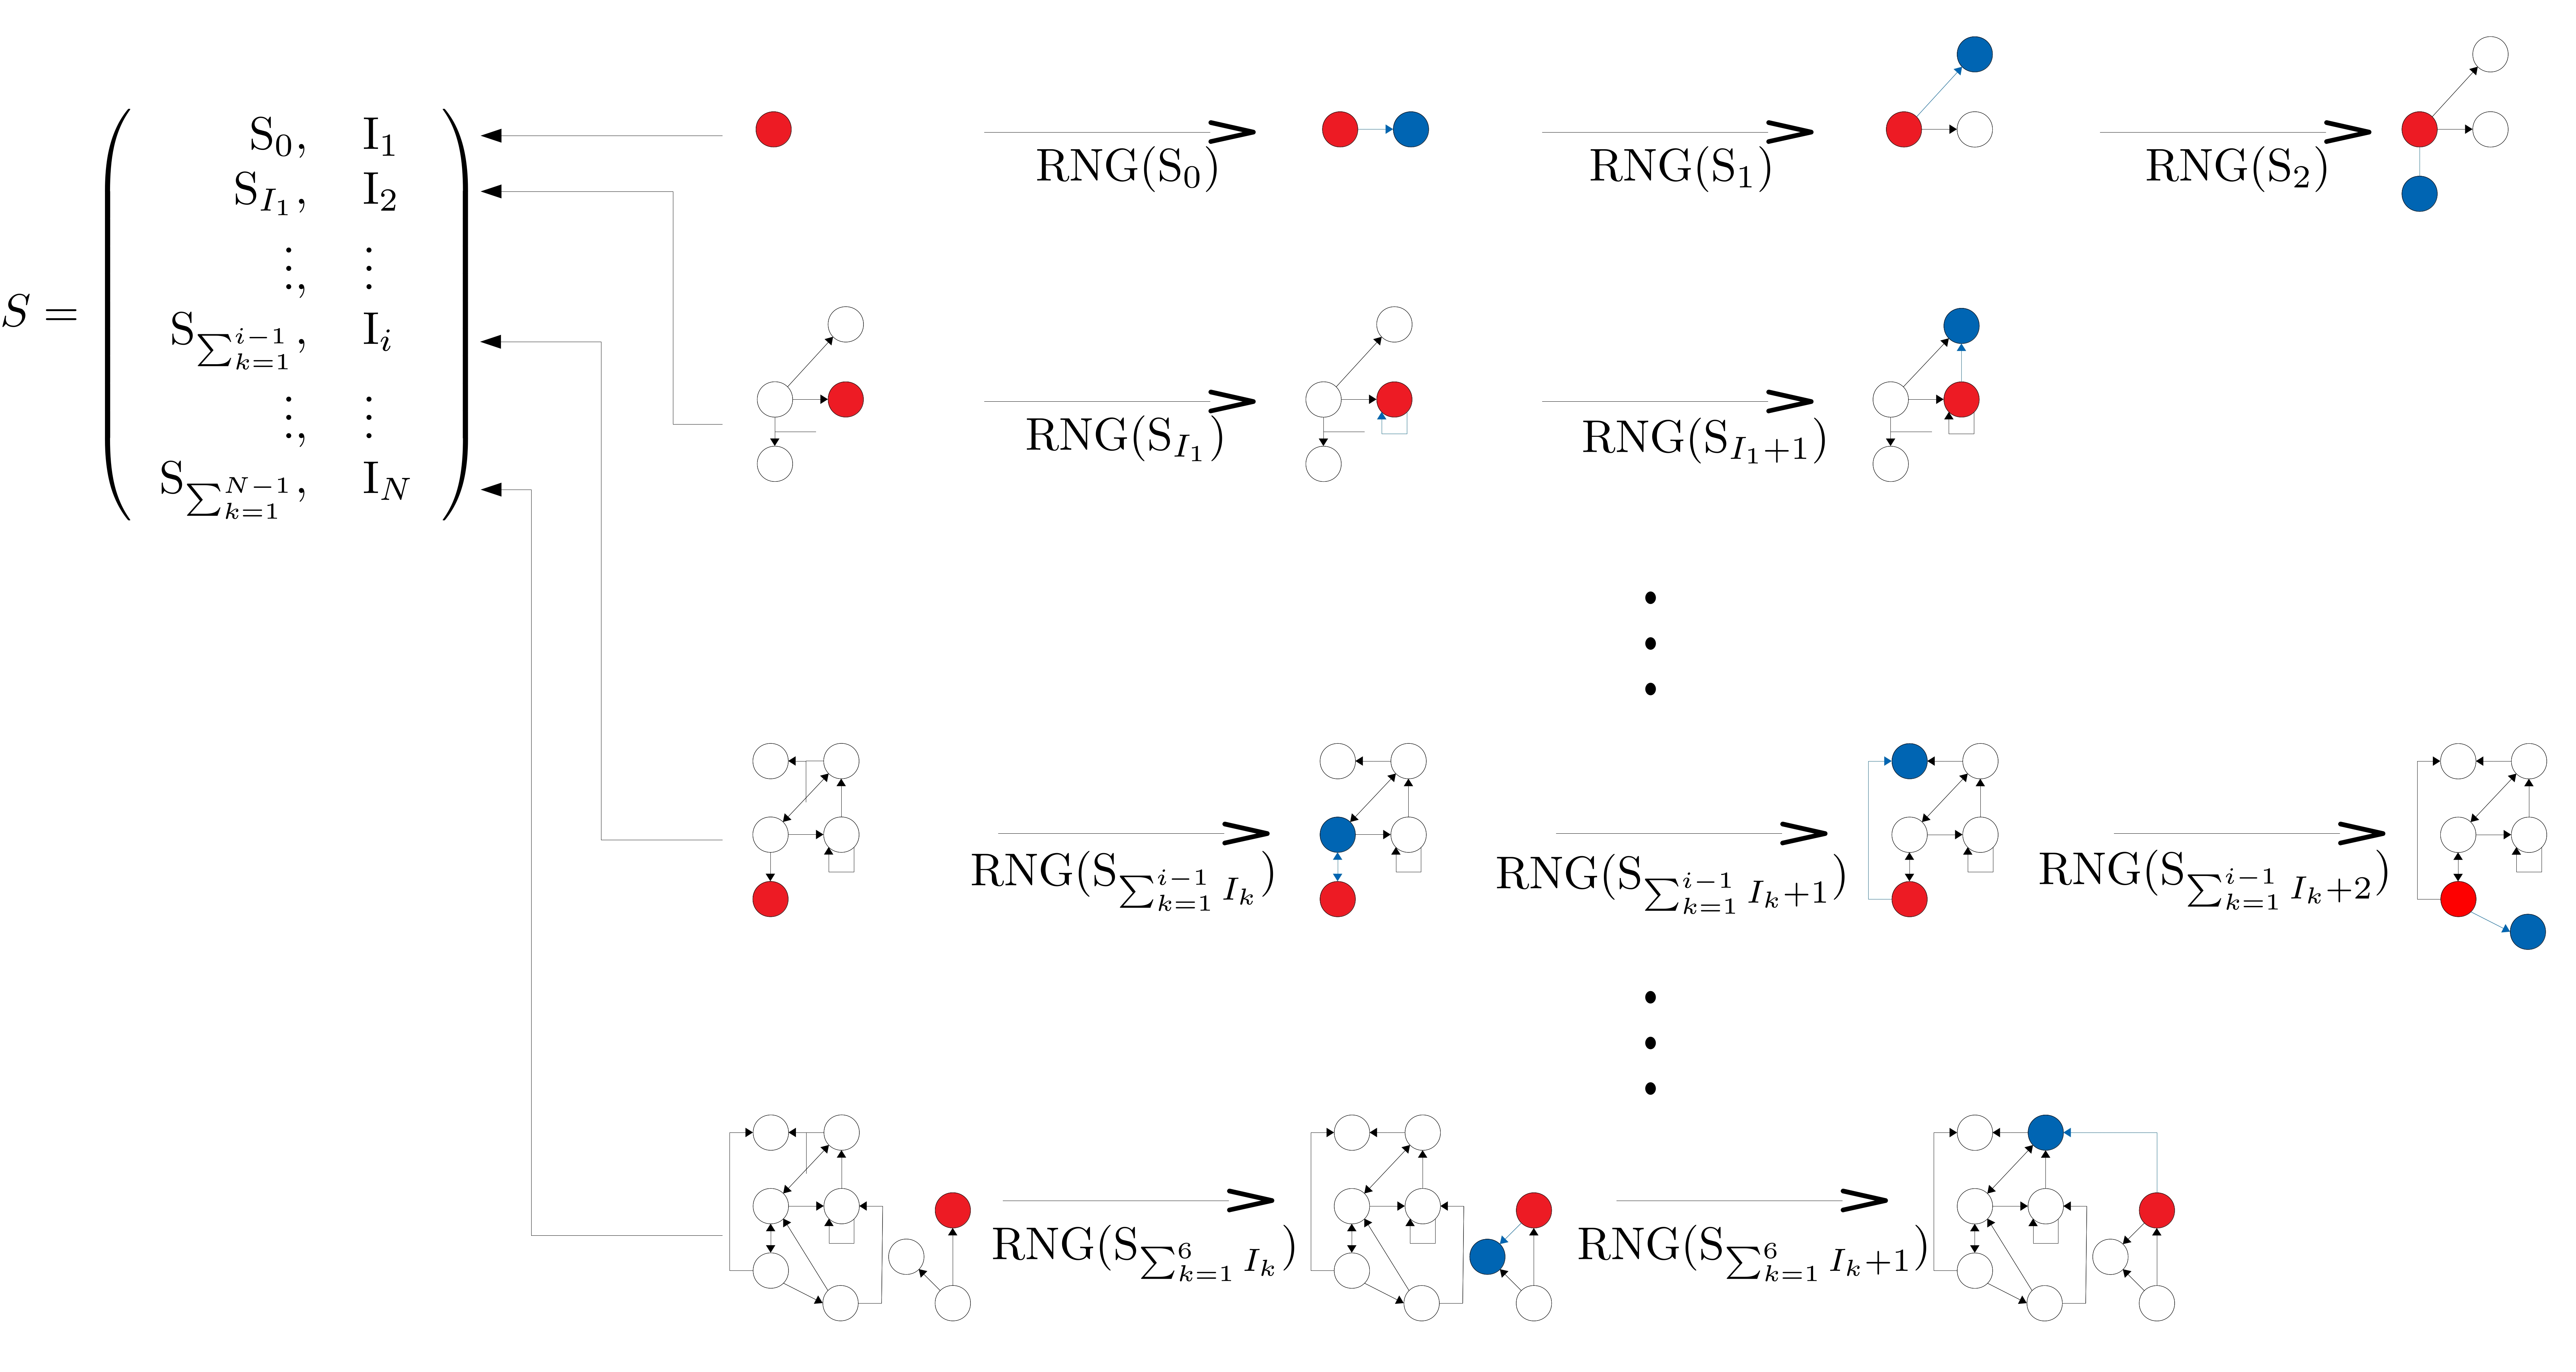
\includegraphics[width=\linewidth]{memory}
				\caption{Construction of graph and vector of states}
				\label{fig:construction}
			\end{figure}
		\end{landscape}
		\begin{landscape}
			\begin{figure}
				\centering
				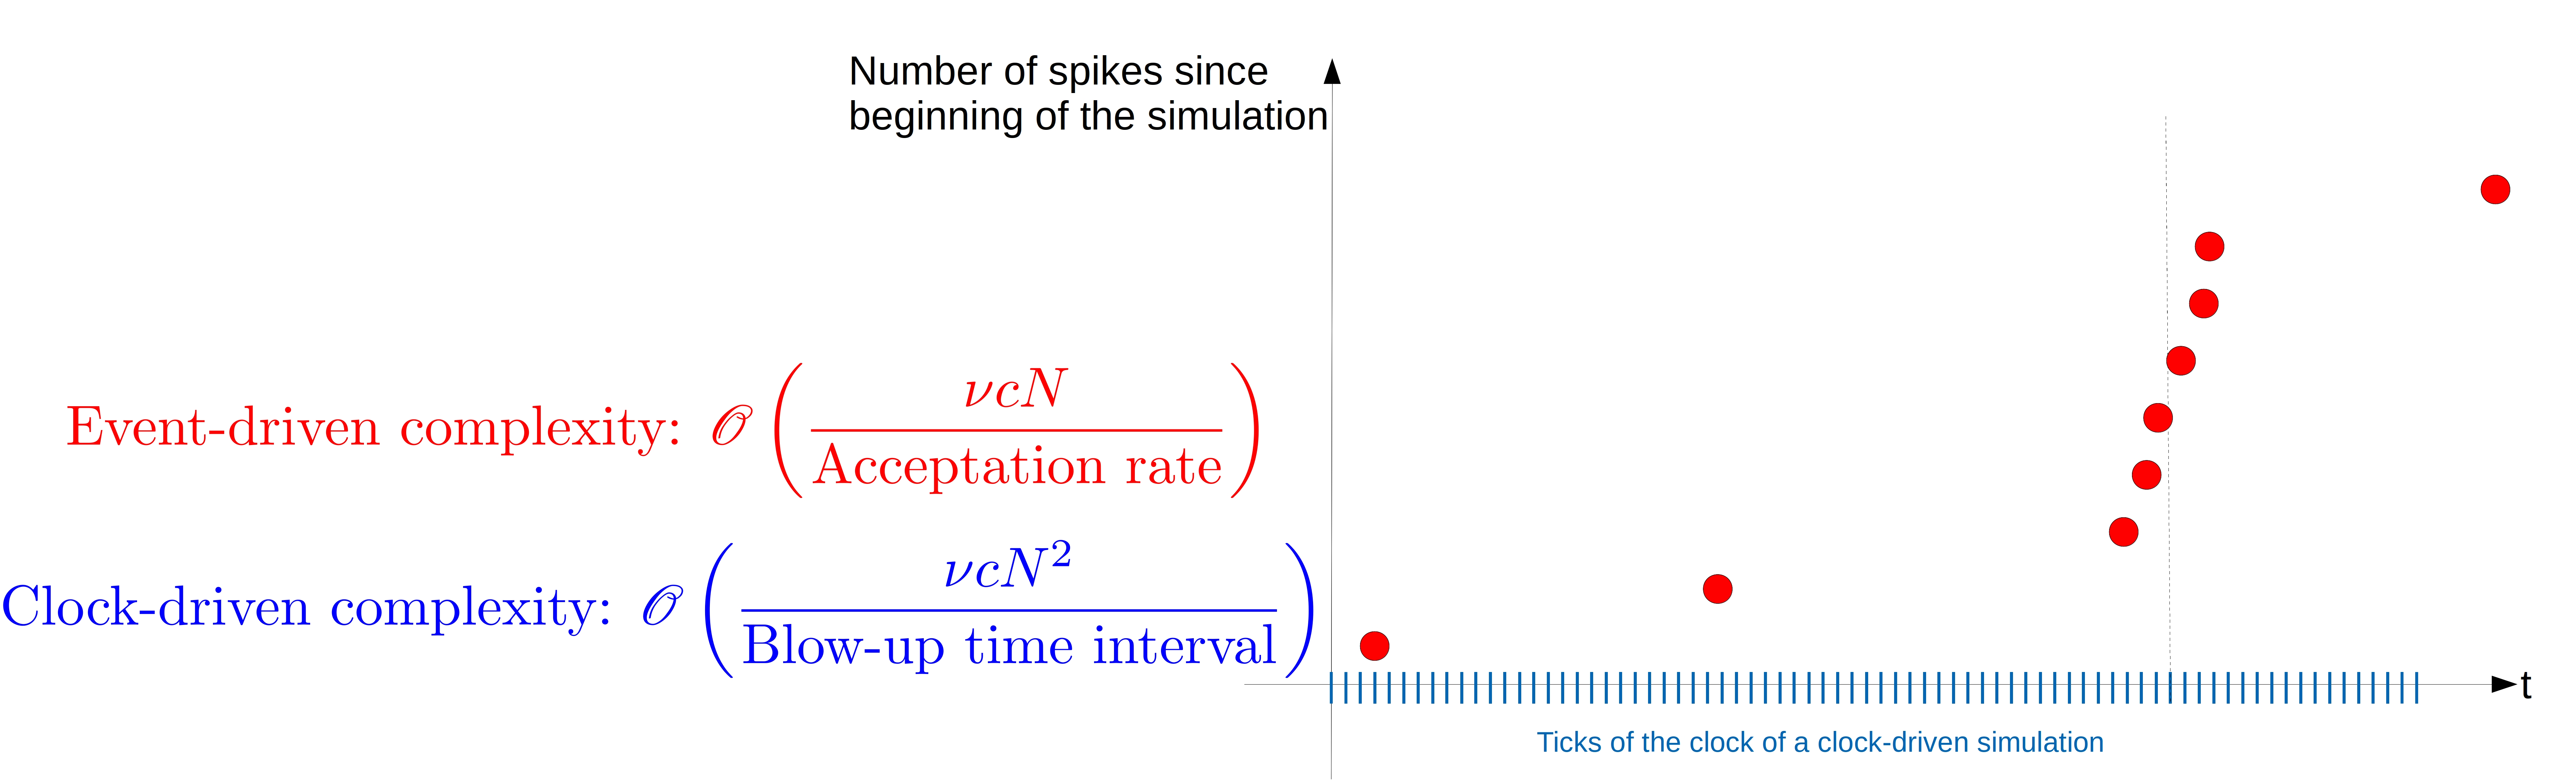
\includegraphics[width=\linewidth]{complexity}
				\caption{Complexity as number of events during a time interval. $\nu$ is a spiking rate, c a connectivity probability and N a number of neurons.}\label{fig:complexity}
			\end{figure}
		\end{landscape}
\end{document}